\documentclass[authordate, rga]{jote-new-article}

\usepackage{caption}

\usepackage{tabularx}

\usepackage{graphicx}

\usepackage{hyperref}

\usepackage[backend=biber,style=apa]{biblatex}

\addbibresource{bibliography.bib}

\jotetitle{The COVID-19 Vaccination Campaign in Switzerland and Its Impact on Disease Spread}
\keywordsabstract{COVID-19, endemic-epidemic modelling, vaccines}
\abstracttext{The objective of this project is to determine the role of vaccines in slowing the spread of coronavirus disease 2019 (COVID-19) in Switzerland incorporating the specific demographics of Switzerland. This work will improve the understanding of the impact of vaccination on the ongoing COVID-19 pandemic. Since 2021, vaccines have been available to prevent severe acute respiratory syndrome coronavirus 2 (SARS-CoV-2, the causative agent of COVID-19) infections in Switzerland but ideal levels of coverage have not yet been achieved. Statistical modelling will be used with epidemiological data to determine the effect unvaccinated or under-vaccinated cantons have on the spread of COVID-19 in other parts of Switzerland as well as the impact of the vaccination strategy used (age-based distribution). Understanding the effect of the lack of vaccination coverage is of strong interest to public health authorities as this is a current issue of mounting concern that needs to be solved. These results will be useful to decision makers. The work will be informed by empirical data from the public health authority–Bundesamt für Gesundheit–and fosters the relationship between the university and the authorities. The project will provide evidence which can be utilised in decision making for vaccination strategy and this funding would allow for the investigation of other aspects of the pandemic than those considered in earlier work by the applicant; namely how insufficient vaccination levels increases cases.}
\runningauthor{Bekker-Nielsen Dunbar}
\jname{Journal of Trial \& Error}
\jyear{2024}
\paperdoi{10.36850/bac3-0248}
\paperreceived{June 17, 2022}
\author[1]{\mbox{Maria Bekker-Nielsen Dunbar\orcid{0000-0002-7249-3524}}}
\affil[1]{OsloMet – Oslo Metropolitan University}
\corremail{\href{mailto:maria.dunbar@uzh.ch}{maria.dunbar@uzh.ch}}
\corraddress{OsloMet – Oslo Metropolitan University}
\runningauthor{Bekker-Nielsen Dunbar}
\paperaccepted{June 23, 2023}
\paperpublished{April 30, 2024}
\paperpublisheddate{2024-04-30}
\jwebsite{https://journal.trialanderror.org}
\rgainfo{TO BE DETERMINED}


\begin{document}
\begin{frontmatter}
  \maketitle
  \begin{abstract}
    \section{Summary (max 2500 characters spaces included)}
    \printabstracttext
  \end{abstract}
\end{frontmatter}






\section{1. Objectives}



In this project, the applicant seeks to analyse COVID-19 data from 2021--2022 to examine the spread of disease in Switzerland, focusing on age, location, and vaccines (pre-exposure pharmaceutical prophylaxis intervention). This is motivated by cases being observed among younger ages in this time period (compared with earlier), with cases also exhibiting spatial heterogeneity in cantons, as well as vaccination rates differing by age group. The applicant is interested in answering questions such as, what is the impact of the current vaccination strategy and how problematic are cantons with low vaccine uptake? To this end, the objectives of this project are:


\begin{itemize}
  \item To assess the role of age and location on the evolution of cases and determine the effect of low vaccination coverage taking such demographic differences into account



  \item To examine the impact of the vaccination strategy chosen by the Swiss public health authorities



  \item To evaluate the usefulness of earlier rollout of vaccination of younger age groups than considered in the original COVID-19 vaccination strategy for Switzerland



  \item To determine the relationship between vaccination strategies, vaccination coverage, and cases and how this is affected by different serotypes of the SARS-CoV-2 virus (variants)


\end{itemize}

\section{2. Background}



Gaining an understanding of the spread of the SARS-CoV-2 virus driving the COVID-19 pandemic is important to determine how to stop disease transmission and prevent excess mortality. Early in the outbreak it was noted that if the disease was not contained it would be expected to become endemic (Begley, 2020; Hamblin, 2020; Wu et al., 2020). The disease has been present in Switzerland for two years. At the end of 2021, Switzerland had observed the greatest number of COVID-19 cases since the beginning of the outbreak in 2020. Pharmaceutical countermeasures in the form of vaccines were approved for use by the Swiss medical authorities at the end of that year. An age-based distribution scheme was used as the vaccine rollout commenced and continued in 2021 with a booster (additional dose of vaccine after immunity is achieved which is used to maintain immunity) included in the immunisation schedule for COVID-19 during 2022. Vaccines were prioritised for those with co-morbidities or underlying conditions and then distributed according to age: those aged 65 years and older were first invited to be immunised, later followed by 16--64 year-olds, and finally 12--15 year-olds. Changes in the age profile of cases (who is getting sick) and distribution of cases (where people are getting sick), with a shift from urban centres to now more rural, unvaccinated communities have been seen compared to earlier, as a result of vaccination rollout. Following a medical authorisation of the vaccines for children in December 2021, as of January 2022, children aged from 5 to 11 have been included in the Swiss vaccination strategy.







Vaccination is not mandatory in Switzerland and pockets of unvaccinated populations have the potential to hamper disease control efforts as they leave susceptible subpopulations who can reignite spread of disease. Waning antibody levels lead to a need for a booster vaccine; however intervention fatigue persists which could lead to less uptake of the booster. Understanding the impact of vaccination is pertinent to understanding the requirements of public health messaging used in the vaccination campaigns to ensure sufficient coverage.







Vaccine hesitancy (defined as a delay in acceptance, or refusal, of vaccines despite availability) is found in Switzerland. The World Health Organization named vaccine hesitancy as one of the ten threats to global health in 2019, noting its detrimental effects on populations who are less protected against life-threatening diseases even in non-pandemic settings. Hesitancy affects the uptake of vaccines and likely also the adherence to other interventions in certain population groups. Dose-



specific (1st, 2nd, booster) vaccination coverage will be used in the work. With increasing numbers of doses required, uptake is expected to decrease due to intervention fatigue. Sub-optimal use of vaccination in the general population (where optimal use would be a vaccine coverage level equal to or above the herd immunity threshold) leaves opportunity for pathogen mutation, which in turn may reduce the effectiveness of the vaccine as a vaccine-escape mutation becomes more likely. In-



formation on disease strain (variants) is available and will be included in modelling as time-varying effect (the proportions of strains circulating). This allows for the evaluation of the vaccination strategy with respect to variants, a question many currently wish to know the answer to. Understanding the impact of various serotypes may help determine the make-up of future polyvalent vaccines for invasive COVID-19 infections.







To support the research objective, the applicant will analyse infectious disease case surveillance data to detect patterns of spread and gain an understanding of the impact of vaccination coverage. The data to be used in this work is extensive and detailed and includes information on cases, age, location (canton), vaccination, virus variant, and testing. The vaccination coverage is time-dependent, age-dependent, and location-dependent, due to the rollout of the vaccine as outlined in



the previous paragraph. The applicant will employ endemic-epidemic modelling to assess the impact of vaccination on the ongoing COVID-19 outbreak in Switzerland. The endemic-epidemic model is a state-of-the-art statistical model for infectious disease surveillance developed by researchers at the University of Zurich (UZH). It has seen myriad applications and increasing use during the COVID-19 pandemic (Bekker-Nielsen, Dunbar \& Held, 2020).







\begin{figure}[t!]
  \begin{fullwidth}
    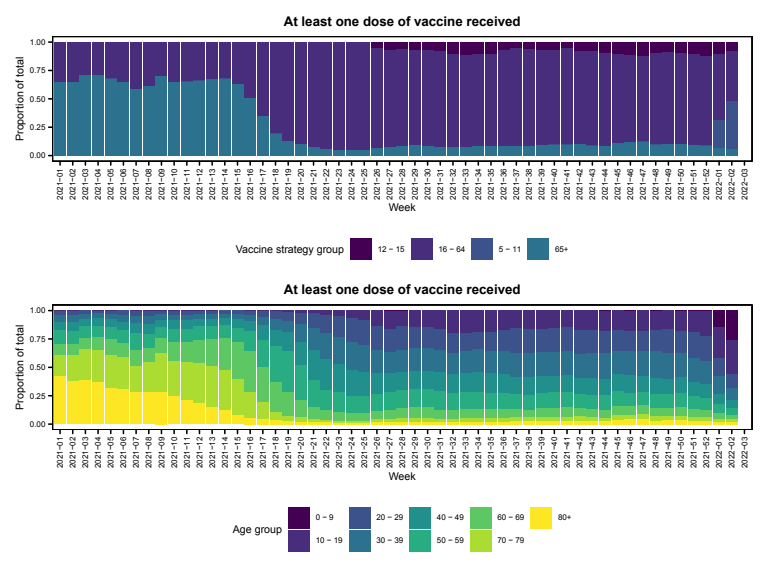
\includegraphics[width=\linewidth]{media/image1.png}


    \caption{Vaccines (first dose) registered given by vaccination strategy (above) and ten-year age bands (below) in Switzerland in 2021 and 2022 (thus far)}

    \label{fig:rId5}
  \end{fullwidth}


\end{figure}



\begin{figure}[t!]
  \begin{fullwidth}
    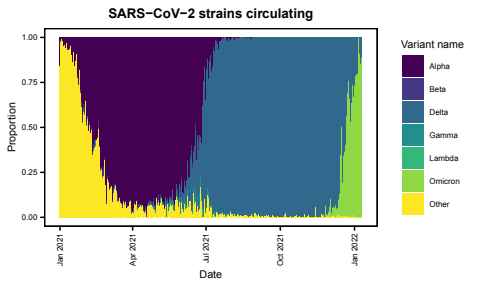
\includegraphics[width=\linewidth]{media/image2.png}

    \caption{Variants registered in Switzerland in 2021 and 2022 (thus far)}

    \label{fig:rId6}

  \end{fullwidth}


\end{figure}










\subsection{2.1 Research background}



Transmission of respiratory pathogens can happen as a result of contacts between an infectious and susceptible person. Including contact matrices (an empirical measure of the amount of normal contact between people based on their ages) in endemic-epidemic models has been shown to improve their performance compared with using simple mixing assumptions (Meyer \& Held, 2016). In previous work on COVID-19, the applicant has successfully examined the option of using time-varying contact matrices in endemic-epidemic models as a way of incorporating social distancing policy, focusing particularly on school closures as schools are a main source of contact for certain age groups (Bekker-Nielsen, Dunbar et al., 2022). For this reason, it will be possible to use the knowledge attained to create a country-wide analysis using similar methodology (the original analysis focused on Zurich). A protocol for the first Switzerland analysis of has been made available by the applicant at DOI:10.17605/OSF.IO/QH3GD. A pre-print of this work (which uses 2020 case data) will be archived and publicly available by the time the funding for this call starts. This manuscript will provide the basis or starting point for the work in this project.







A spatial dispersal power law (which suggests more populated cantons will attract more visitors than less population cantons if the two options are equidistant from the origin) has been shown to improve model performance in endemic-epidemic modelling (Meyer \& Held, 2014). The applicant has included effects of spatial movement in endemic-epidemic models through the use of a power law as well as a gravity model (another measure of attraction in space which posits that mobility increases with population but decreases with distance) (Grimée et al., 2021). For this reason, it will also be possible to use the knowledge attained to create a Switzerland-specific analysis using similar methodology (the original analysis looked at Switzerland and neighbouring regions).






In this work, an age-and-location-dependent endemic-epidemic model will be constructed. Improvement in model performance will be examined through comparison with the previous two model types (just age and just spatial effects). Due to the length of the time scale considered in the work, the applicant intends to include seasonal effects in the modelling efforts. Vaccines have been included in endemic-epidemic modelling (using the log-proportion of all eligible who remain unvaccinated to reflect the size of the susceptible population) (Herzog et al., 2011). This will also be included in the 2021--2022 Switzerland COVID-19 model. The same information (vaccines given) is used to determine vaccination coverage, and this can also be included in the statistical model as a covariate. Calls for other distribution criteria than age to be considered when introducing novel vaccines to immunisation schedules, such as socio-economic status (Mamelund et al., 2021), have been made. Analysis of alternative scenarios is possible in the modelling and has successfully been utilised in the analysis of non-pharmaceutical interventions to evaluate the impact of their timing. Similar approaches have yet to be utilised for assessing the impact of alternative vaccination strategies. For this reason, it will be possible to evaluate the vaccine rollout strategy used in Switzerland. The information required to populate the modelling in this project is publicly available.








\begin{figure}[t!]
  \begin{fullwidth}
    \centering
    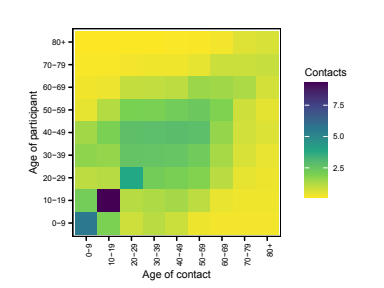
\includegraphics[width=.6\linewidth]{media/image3.png}

    \caption{Contact matrix for Switzerland with the same age groups as in the Bundesamt für Gesundheit data}

    \label{fig:rId7}
  \end{fullwidth}


\end{figure}

\begin{figure*}[b!]
  \begin{fullwidth}
    \centering
    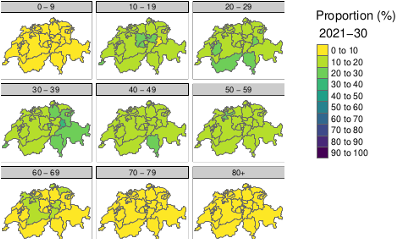
\includegraphics[width=.49\linewidth]{media/image4a.png}
    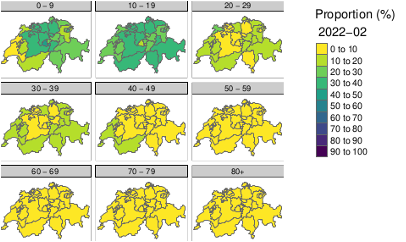
\includegraphics[width=.49\linewidth]{media/image4b.png}

    \caption{Vaccination coverage proportions by age group in ISO week 31 of 2021 and ISO week 2 of 2022 (snapshots of the entire data series)}

    \label{fig:rId8}
  \end{fullwidth}
\end{figure*}

\begin{figure*}[t!]
  \begin{fullwidth}
    \centering
    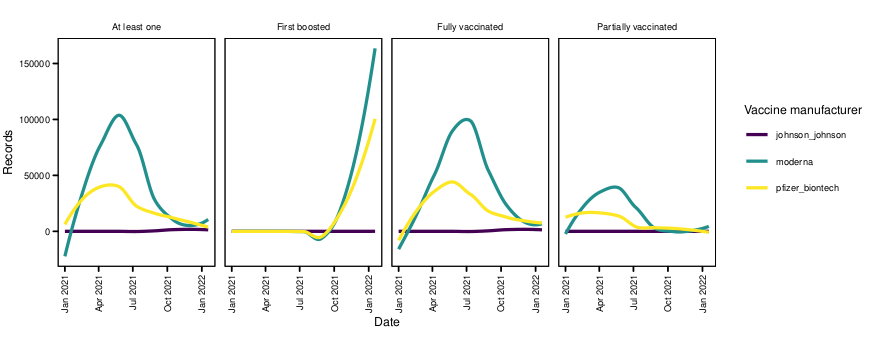
\includegraphics[width=.9\linewidth]{media/image5.png}

    \caption{Vaccines used in Switzerland in 2021 and 2022 (smoothed to show the pattern). Fully vaccinated and partially vaccinated are defined based on the vaccination schedule pre-booster}

    \label{fig:rId9}
  \end{fullwidth}


\end{figure*}




































\section{5 Significance}



Due to the nature of SARS-CoV-2, work on this virus is expected to contribute to the knowledge of other endemic human coronaviruses and respiratory disease outbreaks. COVID-19 is currently the only coronavirus for which there is a vaccine. Other emerging coronaviruses resulting in severe pneumonia in humans, such as SARS and MERS, can also spread from human-to-human transmission and their control may benefit from the results of this work. The topic of this project supports the International Health Regulations (World Health Organization, 2016) as well as the World Health Organizations strategic goals (World Health Organization, 2019) and research agenda on health emergencies.







This project will increase the image of University of Zurich internationally which has an impact on its standing. Adding to the publications on endemic-epidemic models strengthens the evidence base for the use of such modelling in routine and special infectious disease surveillance. Previous results using this modelling approach for COVID-19 have already been published in prominent scientific journals and presented at international conferences and work from this project is also expected to be



highlighted among scientific peers. The work is of value to public health personnel who advise policy makers on public health decision making.



\newpage
\section{References}

\hspace*{\parindent}Begley, S. (2020, Feb 4). Experts envision two scenarios if the new coronavirus isn't contained. \emph{Stat News}. \url{https://www.statnews.com/2020/02/04/two-scenarios-if-new-coronavirus-isnt-contained/}


Bekker-Nielsen Dunbar, M., \& Held, L. (2020). Epidemic-endemic framework used in COVID-19 modelling. \emph{REVSTAT}, \emph{18}(5). https://www.ine.pt/revstat/pdf/REVSTAT\_v18-n5-02.pdf


Bekker-Nielsen Dunbar, M., Hofmann, F., \& Held, L. (2022). Assessing the effect of school closures on the spread of COVID-19 in Zurich. \emph{To Appear in an Issue of Journal of the Royal Statistical Society Series A Dedicated to the Special Topic Meeting on Covid-19 Transmission (Held in 2021)}. \url{https://rss.org.uk/RSS/media/File-library/News/2021/BekkerNielsenHeld.pdf}


Grimée, M., Bekker-Nielsen Dunbar (joint first), M., Hofmann, F., \& Held, L. (2021). Modelling the effect of a border closure between Switzerland and Italy on the spatiotemporal spread of COVID-19 in Switzerland. \emph{Spatial Statistics}, 100552. \url{https://doi.org/10.1016/j.spasta.2021.100552}


Hamblin, J. (2020). You're likely to get the coronavirus: Most cases are not life-threatening, which is also what makes the virus a historic challenge to contain. \emph{The Atlantic}. \url{https://www.theatlantic.com/health/archive/2020/02/covid-vaccine/607000/}


Herzog, S. A., Paul, M., \& Held, L. (2011). Heterogeneity in vaccination coverage explains the size and occurrence of measles epidemics in German surveillance data. \emph{Epidemiology and Infection}, \emph{139}(4), 505--515. \url{https://doi.org/10.1017/S0950268810001664}


Mamelund, S.-E., Shelley-Egan, C., \& Rogeberg, O. (2021). The association between socioeconomic status and pandemic influenza: Systematic review and meta-analysis. \emph{PLOS ONE}, \emph{16}(9), 1--31. \url{https://doi.org/10.1371/journal.pone.0244346}


Meyer, S., \& Held, L. (2014). Power-law models for infectious disease spread. \emph{The Annals of Applied Statistics}, \emph{8}(3), 1612--1639. \url{https://doi.org/10.1214/14-AOAS743}


Meyer, S., \& Held, L. (2016). Incorporating social contact data in spatio-temporal models for infectious disease spread. \emph{Biostatistics}, \emph{18}(2), 338--351. \url{https://doi.org/10.1093/biostatistics/kxw051}


World Health Organization. (2016). \emph{International Health Regulations (2005) }(3\textsuperscript{rd} ed.). \url{https://www.who.int/ihr/publications/9789241580496/en/}


World Health Organization. (2019). \emph{Thirteenth General Programme of Work 2019--2023}. \url{https://apps.who.int/iris/bitstream/handle/10665/324775/WHO-PRP-18.1-eng.pdf}


Wu, J. T., Leung, K., \& Leung, G. M. (2020). Nowcasting and forecasting the potential domestic and international spread of the 2019-nCoV outbreak originating in Wuhan, China: A modelling study. \emph{Lancet}, \emph{395}(10225), 689--697. \url{https://doi.org/10.1016/S0140-6736(20)30260-9}









\end{document}